% En este capitulo se presentan y analizan los resultados experimentales de la
% solucion para el problema de al exploracion multirobot coordinada que fue
% desarrollada en este proyecto.

% Las pruebas realizadas se separan en tres secciones segun su proposito. La
% primera estudia el impacto de construir el GVD de forma incremental. La
% segunda compara las diversas tecnicas de identificacion de objetivos. Y la
% tercera analiza la influencia de las diversas formas de considerar el espacio
% desconocido. 


% Las pruebas realizadas tienen  propositos,  para estudiar el impacto de
% construir el GVD de forma incremental. Para comparar las diversas tecnicas de
% identificacion de objetivos. Y finalmente para analizar la influencia de las
% diversas formas de considerar el espacio desconocido. 

% , se presentan los resultados obtenidos y analizan
%  los resultados los cuales son analizados.

% Comentar que estos son cosas generales a todas las pruebas, que en cada una de
% las siguientes secciones se cambian paramtros aislados con el proposito de
% comparar su impacto. (ver capaz que crierios se van a comparar en cada una)

% generales de las pruebas realizadas. Estas 

Este capitulo esta dedicado a describir las pruebas realizadas y analizar los
resultados obtenidos. Las pruebas se ejecutaron de forma simuladas y consisten
en resolver una instacia del problema de la exploracion multirobot coordinada
con distintas soluciones.
Los resultados de las pruebas separan en cuatro secciones segun su proposito.
En la seccion \ref{sec:exp:cubcal} se evaluan los mapas contruidos en las
purebas. En la seccion \ref{sec:exp:inc} se estudia el impacto de construir el
GVD de forma incremental. En la seccion \ref{sec:exp:idobj} se compara las
diversas tecnicas de identificacion de objetivos. Y finalmente, en la seccion
\ref{sec:exp:desco} se analiza la influencia de las formas de considerar el
espacio desconocido. 

\section{Especificación de las pruebas}

A lo largo de esta seccion se especifican las pruebas realizadas en este
proyecto.

% * Pruebas realizadas, cosas generales:
%   * simulador
%   * hardware (de mi pc)
%   * Los robots utilizados
%     * sensor 
%     * robot en si
%   * El entorno de pruebas
%   * Criterios utlizados para analizar los resultados: 
%     * Referencias
%     * Explicar cuales son
%   * Cantidad de pruebas, promedio y varianza

% cuyos resultados se
% presentan a lo largo del capitulo.

% En esta seccion se plantean las caracteristicas generales que comparten todas
% las pruebas que se presentan a lo largo del capitulo.

% En lo que resta de esta seccion se especifican las caracteristicas de las
% pruebas llavadas a cabo. 

% A lo largo del capitulo se presentan diversas pruebas que buscan comparar ciertos
% aspectos de la solucion desarrollada en este proyecto. En esta seccion se
% especifican las caracteristicas generales que comparten todas las pruebas
% realizadas.

% En esta sección se establecen als car


% \subsection{Tipos de prueba}
% El proposito de las pruebas presentadas es evaluar el desempeño de diversos aspectos de una
% solucion al problema de la exploción multirobot. 
% Los tipos de prueba quedan definidos 

% Las pruebas tienen como proposito validar las variantes presentadas para la
% solucion de diviersos aspectos de la del problema de exploracion multirobot.
 
% Para lograr esto se definen pruebas consisten en reslover una instancia de
% dicho problema, cambiando la forma de resolver cada aspecto a validar.

% La instancia del problema de exploracion a resolver es el de explorar un
% entorno cerrado con una flota de robots, hasta que no exista espacio sin
% explorar.

% Debido a esto
% las pruebas se dividen en tres secciones, dependiendo del aspecto que se busca comparar.
% Dado esto las pruebas

% En la seccion \ref{sec:exp:inc} se compara la construccion incremental del GVD contra
% la no incremental, en la seccion \ref{sec:exp:idobj} se
% comparan los metodos de identificación de objetivos que se describen en la seccion
% \ref{sec:pc:idobj}, finalmente en la seccion 
%  la seccion \ref{sec:exp:desco} analiza la
% influencia de las diversas formas de considerar el espacio desconocido. 

% de objetivos que
% utiliza directamente las fronteras como objetivos, con las que se basan en
% simplicar dichas fronteras, tanto la simplificacion basada en K-Means, como la
% basada en cubrimiento. 

% Dado que se quiere comparar la utilidad entre las variantes para ciertas partes de
% la solución, se definen tipos de prueba según las variantes utilizadas. 
% En esta sección se describe el tipo de prueba que se denominara como $base$. Este consiste
% en una solucion del problema de exploracion multirobot que 
 % La solución base consiste en resolver la
% asignación de tareas basada en cubrimiento (seccion \ref{subsec:MiSimp}). La as La construccion de GVD
% incremental como es comentada en \ref{sec:MiConstGVD} con

\subsection{Simulador}
Las pruebas fueron simuladas con Gazebo \cite{gazebo}, el cual fue elegido a
partir del analisis comparativo entre varios simuladores candidatos realizado
en la sección \ref{sec:sim}). 

\subsection{Tipos de pruebas}
Las pruebas tienen como proposito validar ciertos aspectos de la
solucion al problema de exploracion multirobot propuesta en este proyecto.
 
Para lograr esto se define caso de prueba que permite evaluar el desempeño de
una solucion que resueve dicho problema. El caso de pruebas definido consiste
en reslover una instancia de dicho problema, especificamente en explorar un
entorno cerrado con una flota de robots, hasta que no exista espacio sin
explorar. El tipo de mapa generado en la exploración es una grilla de ocupacion
de un tamaño fijo suficiente para representar el entrono explorado.

Para poder validar los aspectos, se prueba la solución propuesta cambiando
unicamente el aspecto a validar. Los aspectos a validar son: la construccion
incremental del GVD (sección \ref{sec:MiConstGVD}). La identificación de
objetivos que simplifica las fronteras basandose en el cubrimiento (seccion
\ref{subsec:MiSimp}). Y la consideracion del espacio desconocido al construir
el GVD presentada en la seccion \ref{subsec:espDesc}, donde las celdas
desconocidas no propagan olas y el conjunto $\mli{UF}$ de celdas desconocidas
que son adyacentes a celdas conocidas pertenecen a generadores ($\mli{UF}
\subseteq \mli{CGen}$).

% Para validar la construccion incremental del GVD esta se compara contra la
% construccion no incremental. En el caso de la identificación de objetivos se
% comparan las tres estrategias propuestas en la seccion \ref{sec:pc:idobj}: el
% identificar las fronteras como objetivos, simplicar dichas fronteras a partir
% K-Means, y simplificarlas basandose en el cubrimiento. Por ultimo, la
% consideracion del espacio desconocido en la contruiccion del GVD se valida
% comparandola contra considerar que el espacio desconocido es libre. 
Para validar la construccion incremental del GVD esta se compara contra la
construccion no incremental. En el caso de la identificación de objetivos esta se
comparan contra identificar todas las fronteras como objetivos, y la tecnica
que obtiene los objetivos simplicando dichas fronteras a partir K-Means. Por
ultimo, la consideracion del espacio desconocido en la contruiccion del GVD se
valida comparandola contra considerar que el espacio desconocido es libre. 

Se evaluan entonces cinco soluciones, la que utiliza todos los aspectos a
validar a la vez, y cada una de las que cambian uno de dichos aspectos.

Con el motivo de probar distintas cargas computacionales, cada prueba se repite
cambiando la granularidad de la grilla de ocupacion utlizada para representar
el entorno explorado. La granularidad se indica a traves de las celdas de una
grilla que se corresponden con un metro cuadrado de la realidad. Los valores de
granularidad utilizados para las pruebas son $1,4,9$ y $16$ celdas
por metro cuadrado ($\frac{celdas}{m^2}$). 

Adicionalente debido a que es posible que ejecuciones de un misma simulacion
lleven a distintos resutlados, con el fin de obtener resultados
estadísticamente significativos cada prueba fue ejecutada 20 veces. Siendo 
$5*4*20=400$ el total de pruebas ejecutadas.
% las tres tecnicas, identfica todas las fornteras como objetivos, 

% Debido a esto
% las pruebas se dividen en tres secciones, dependiendo del aspecto que se busca comparar.
% Dado esto las pruebas

% Para cumplir con la hipotesis (IV) planteada en \ref{sec:hip}
\subsection{Entorno}
Las pruebas se realizan en un entrono cerrado que tiene un area explorable de
aproximadamente $10000m^2$. El entorno esta estructurado en habitaciones,
puertas y corredores de varios tamaños. Los unicos obstaculos presentes en él
son paredes y los mismos robots que pueden obstaculizarse entre
sí. Un mapa de este entrono se muestra en la figura
\ref{fig:willow}.

\begin{figure}[H]
  \center
  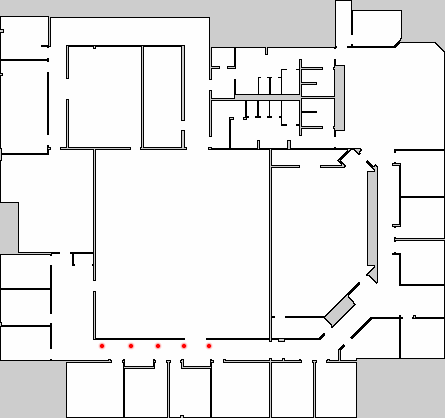
\includegraphics[width=0.5\linewidth]{imagenes/willow/0_250000mRobots2.png}
  \caption[Mapa del entrono utilizado en las pruebas.]{Mapa del entrono utilizado en las pruebas. En negro se indican las paredes, en blanco el espacio libre y en gris el espacio inaccesible. Las posiciones iniciales de los robots se indican en rojo.}
  \label{fig:willow}
\end{figure} 

El entorno fue construido a partir de un modelo que se encuentra disponible por
defecto en Gazebo, llamado \say{Willow Garage}, el cual se modifico para
reducir el area a exporar y que sea cerrado (sin salidas al exterior).

\subsection{Robots}
Los robots simulados\footnote{Especificación disponible en línea:
\url{https://gitlab.fing.edu.uy/federico.ciuffardi/pioneer_p3dx_model}} en las
pruebas modelan al robot diferencial Pioneer 3-DX \cite{p3dx} (figura
\ref{fig:p3dx}). Cada robot esta equipado con un sensor LiDAR basado en el
modelo URG-04LX-UG01 \cite{hokuyo}, que permite tomar medidas de distancia de
hasta $5.6m$, utilizando una frecuencia de $10hz$ de un maximo de $36hz$.
Adicionalente el sensor fue alterado para tomar medidas en los $360$\textdegree
al rededor del robot y para proporcionar medidas perfectas (sin ruido).

\begin{figure}[H]
  \centerfloat

  \subfloat[Real.]{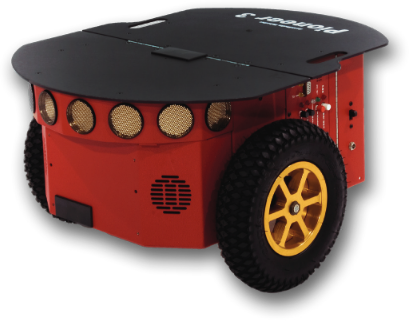
\includegraphics[clip=true, width=0.33\textwidth]{imagenes/pion/real.png}}
  \qquad
  \subfloat[Simulado.]{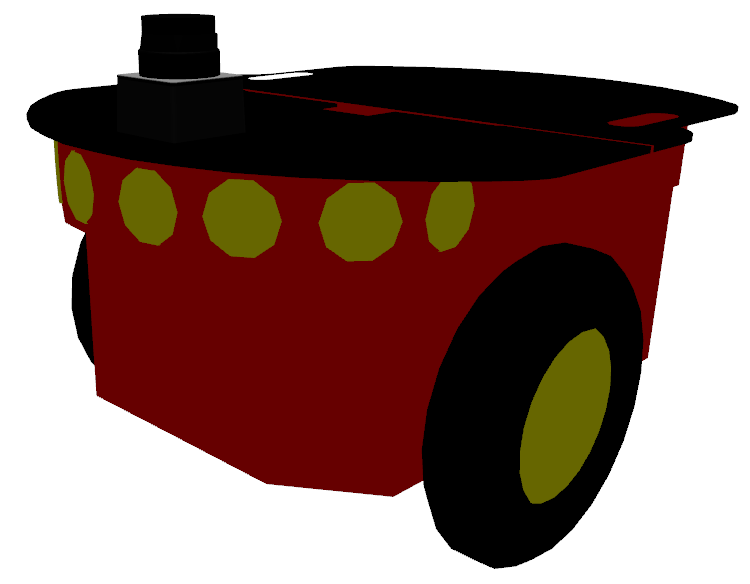
\includegraphics[clip=true, width=0.33\textwidth]{imagenes/pion/sim.png}}

  \caption[Robot diferencial Pioneer 3-DX.]{Robot diferencial Pioneer 3-DX.}\label{fig:p3dx}
   % A la izquierda se muestra el robot real, y a la derecha su version simulada.

\end{figure}

La flota de exploración se compone de cinco robots, ubicados en las posiciones
indicadas en la figura \ref{fig:willow}. Las comunicaciones entre los robots de
la flota son sin perdida y de rango infinito.

\subsection{Software}
El software utilizado en las pruebas fue Ubuntu \emph{20.04}, ROS \emph{Noetic} y Gazebo
\emph{11.5.1}. 

\subsection{Hardware}
El simulador junto al resto de procesos necesarios para llevar a cabo una
prueba fueron ejecutados en una computadora personal equipada con un procesador
Intel Core i3-9100F, un procesador gráfico GeForce GTX 660 y 16GB de memoria
RAM.

\section{Metricas}
Con el proposito comparar cuantitativamente los resultados de las pruebas se
establece un conjunto de metricas. 

Una parte de las metricas utlizadas se proponen en \cite{yan2015metrics} y
evaluan el problema de exploración en general, estas son: \emph{tiempo de
exploración}, \emph{distancia total recorrida por la flota}, \emph{completitud
del mapa} y \emph{calidad del mapa}. 

El \emph{tiempo de exploración} refiere al tiempo desde que los robots
comienzan con la primera asignación de tareas (seccion \ref{sec:asigTar}) hasta
que no se detecta mas espacio desconocido por explorar y se da por terminada la exploración.

La \emph{distancia total recorrida por la flota} es la suma las distancias
recorridas por cada robot de la flota a lo largo de la exploración. En
\cite{yan2015metrics} esta metrica se presenta como \emph{costo de
exploración}, ya que los autores la consideran como una buena aproximación del
costo energetico del robot. 

 % mapas de referencia para evaluar los mapas resultantes de las pruebas,

Para calcular las metricas de \emph{completitud} y \emph{calidad} de los mapas
es necesario contar con mapas de referencia considerados como correctos. En
este proyecto estos se representan a traves de grillas de ocupacion al igual
que los generados en la exploración. Se definen cuatro mapas de
referencia, uno por cada nivel de granularidad utlizado en las pruebas, con el
proposito de poder comparar cualquiera de los mapas obtenidos en pruebas con
un mapa de referencia de igual granularidad. Los mapas de referencia se pueden
apreciar en la figura \ref{fig:mref}. 

\begin{figure}[H]
  \centerfloat

  \subfloat[$1  \frac{celda}{m^2}$]{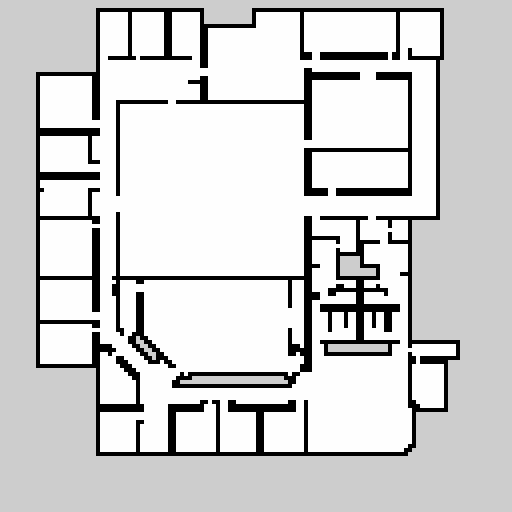
\includegraphics[clip=true, width=0.22\textwidth]{imagenes/willow_ref/1_000000m.png}}
  \qquad
  \subfloat[$4  \frac{celda}{m^2}$]{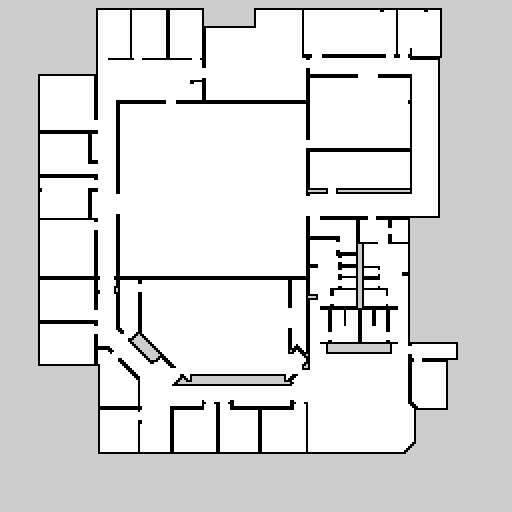
\includegraphics[clip=true, width=0.22\textwidth]{imagenes/willow_ref/0_500000m.png}}
  \qquad
  \subfloat[$9\frac{celda}{m^2}$]{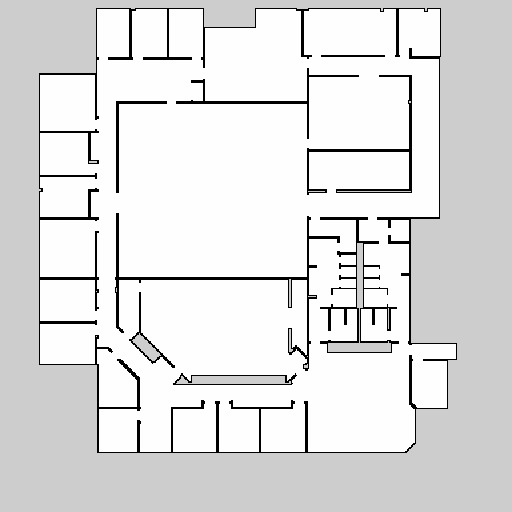
\includegraphics[clip=true, width=0.22\textwidth]{imagenes/willow_ref/0_333333m.png}}
  \qquad
  \subfloat[$16 \frac{celda}{m^2}$]{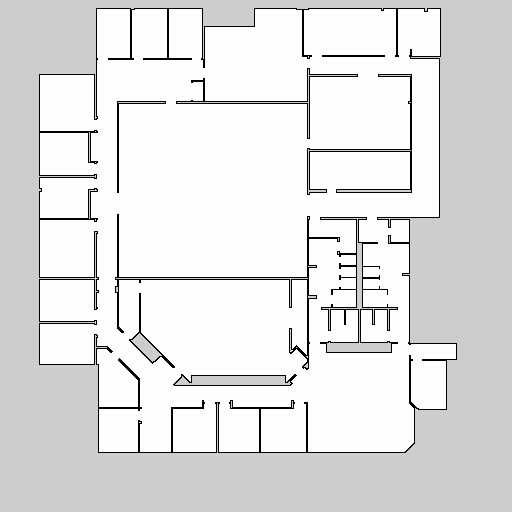
\includegraphics[clip=true, width=0.22\textwidth]{imagenes/willow_ref/0_250000m.png}}

  \caption[Mapas de referencia utlizados.]{Mapas de referencia utlizados. En negro se indican las paredes, en blanco el espacio libre y en gris el espacio desconocido por ser inaccesible.}\label{fig:mref}
   % A la izquierda se muestra el robot real, y a la derecha su version simulada.

\end{figure}

Notar que existe espacio desconocido en los mapas de referencia, esto se debe a
que la grilla de ocupación no se ajusta al espacio explorable. En terminos de
las metricas calculadas, el espacio desconocido en los mapas de referencia no es
considerado como parte de los mapas, tanto en los mapas de referencia como en
los obtenidos en las pruebas.

% Es decir las unicas celdas que se consideran como
% parte de los mapas al calcular las metricas son las que tienen un estado
% distinto a desconocido en los mapas de referencia.
% De
% esta forma los mapas de referencia no contienen celdas desconocidas, a
% diferencia de los mapas resultantes de las pruebas los cuales si pueden.

La \emph{completitud del mapa} se define segun (\ref{eq:metComp}) donde
$M_{exp}$ es el area conocida del mapa obtenido en la exploración y $M_{ref}$
es el area del mapa de referencia.

\begin{equation} \label{eq:metComp}
completitud\ del\ mapa = \frac{M_{exp}}{M_{ref}}
\end{equation}

La \emph{calidad del mapa} se establece en (\ref{eq:metCal}) donde se introduce
$E_{exp}$ equivalente al área ocupada por las celdas del mapa obtenido en
la exploración cuyo estado difiere del estado de su celda correpondiente en el
mapa de referencia.

\begin{equation} \label{eq:metCal}
calidad\ del\ mapa = \frac{M_{exp}-E_{exp}}{M_{ref}}
\end{equation}

El resto de las metricas fueron diseñadas especificamente para
este proyecto, estas son: \emph{tiempo promedio en construcción de GVD}, \emph{porcentaje
del tiempo de obtención de información en el que se construye el GVD}, \emph{tiempo
promedio en identificación de objetivos} y \emph{porcentaje promedio del tiempo de
obtención de información en el que se identifican los objetivos}.

El \emph{tiempo promedio en construcción de GVD} es el promedio del tiempo que
toma construir el GVD en las etapas de obtención de información en cada
asignación de tareas (seccion \ref{sec:asigTar}).

El \emph{porcentaje del tiempo de obtención de información en el que se
construye el GVD} es el resultado de multiplicar por $100$ a la division entre
suma del los tiempos que toma construir el GVD en las etapas de obtención de
información y la suma de los tiempos que llevan las etapas de obtención de
información.

El \emph{tiempo promedio en identificación de objetivos} y el \emph{porcentaje
promedio del tiempo de obtención de información en el que se identifican los
objetivos} son metricas analogas a las dos ultimas, pero refieren a la
identificación de objetivos en lugar de la construcción del GVD.

\section{Resultados}
\newlength{\graphlen}
\setlength{\graphlen}{0.75\textwidth}


Los resultados explerimentales obtenidos son presentados y analizados en esta
seccion. Las tablas que se presentan a lo largo de la sección indican para cada
prueba los promedios y desviaciones estandar de las metricas en las 20
repeticiones que se hacen debido al no determinismo del simulador.

\subsection{Cubrimiento y calidad de los mapas} \label{sec:exp:cubcal}
% Capaz aca puedo mencionar lo que pasa con los errores

% el cubrimiento y la completitud: completitud mayor a 0.999 para todas combinaciones de granularidades y soluciones probadas

% el error y la calidad:

En la tabla \ref{tab:todo3} se muestra la completitud y calidad de los mapas
obtenidos en todas las pruebas realizadas. 

Con respecto a la completitud es posible apreciar que no existen diferencias
mayores entre las variantes de la implemetnación, teniendo todos los mapas
generados una completitud alta. Dado que el criterio de parada es que no se
detecte mas espacio por explorar, estos valores hablan principalmente de la
capacidad de detectar el espacio desconocido explorable que tienen las
soluciones. Todas las soluciones detectan expacio desconocido explorable
mientras exista una un celda $c_1$ libre y otra $c_2$ desconocida tal que $c_1
\in ady_4(c_2)$ (seccion \ref{subsec:Grilla}), principalemente porque en estas
condiciones se asume que los robots no pueden atravezar de $c_1$ a $c_2$. Dicho
esto se presume que la completitud de los mapas no es perfecta debido a la
presencia de celdas ubicadas en esquinas de paredes que que a pesar de no
cumplir con las codiciones de ser detectadas como explorables, lo son. Un
ejempo de este tipo de celda se muestra en la figura \ref{fig:faltaCub}. Sin
embargo los valores de completitud obtenidos indican que este tipo de
situaciones son despreciables.

\begin{figure}[H]
  \centerfloat

  \subfloat[Mapa de referencia.]{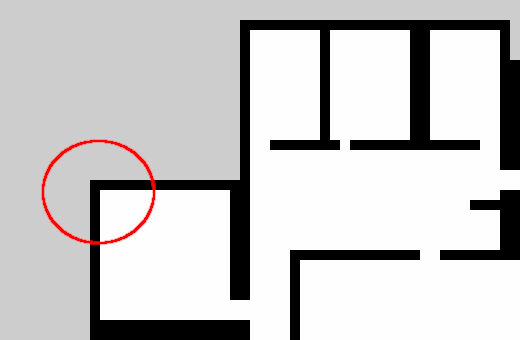
\includegraphics[clip=true, width=0.33\textwidth]{imagenes/faltaDeCub/ogred.png}}
  \qquad
  \subfloat[Mapa generado.]{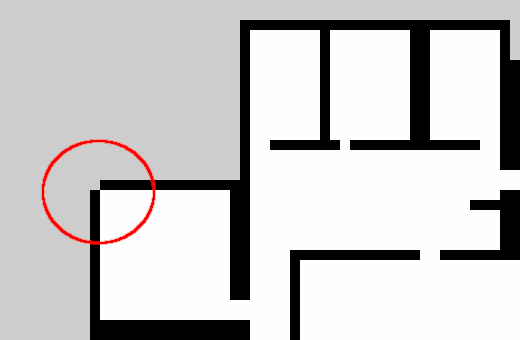
\includegraphics[clip=true, width=0.33\textwidth]{imagenes/faltaDeCub/faltaCubRed}}

  \caption{Esquina superior izquierda del mapa referencia y de uno de los mapas
  obtenidos en las pruebas que presenta una celda explorable que no se reconoce
como tal. Ambos mapas corresponden a una granularidad de una celda por metro cuadrado.}\label{fig:faltaCub}
   % A la izquierda se muestra el robot real, y a la derecha su version simulada.

\end{figure}

Los resultados de calidad de los mapas obtenidos son similares a los de
completitud, los mapas contruidos tienen una calidad alta, sin existir
diferencias significativas entre las variantes. Esto es esperable ya que
los sensores simulados fueron configurados para proporcionar medidas perfectas.
Aunque a pesar de esto la calidad no perfecta, esto puede se explica en primer
lugar por el impacto de la completitud del mapa en su calidad. En segundo lugar
por la existencia de varios robots que pueden detectase como obstaculos entre
sí, generado celdas obstaculizadas que no se encuentran en el mapa de
referencia. Y en tercer lugar porque a pesar de las configuración de los
sensores, sus medidas tienen un ruido pequeño.

Estos resultados de completitud y calidad del mapa permiten concluir que todas
las variantes logran resolver de manera satisfactoria el problema de la
exploración multirobot, en terminos de los mapas contruidos. Las
siguientes secciones se dedican a discutir los impactos que las diferentes
variantes en terminos de tiempo y costo de exploracion.

% De la
% equacion 4 se de deduce que el cubrimiento siempre es mayor o igual que la
% calidad. Por lo tanto 


%%%%%%%%
% Dado que las diferencias son despreciables se puede
% concluir que el impacto de el uso de las distintas tambien despreciable.

% confirman que todas las variantes de la implemetnacion 
% finalizar su ejecucion con un mapa casi completo del entorno.

% Estos resutlados son los esperados ya que
% la mision concluye al no quedar mas espacio por explorar.

% Es posible apreciar que todos los
% mapas cubren casi en su totalidad al entorno y que la calidad de dichos mapas
% es casi perfecta en todos los casos.

\begin{table}[H]
%29/12/2021 18:15:43
\hbadness = 10000
\tolerance=9999
\emergencystretch=10pt
\hyphenpenalty=10000
\exhyphenpenalty=100
\begin{center}

% \begin{adjustbox}{minipage=0.75\paperwidth, center}
\begin{adjustbox}{width=1\textwidth}
\small

\begin{tabularx}{\textwidth}{|X|C{0.80cm}|X|X|}

\hline
Variante & $\frac{celdas}{m^2}$ & Completitud del mapa & Calidad del mapa \\ \hline\hline
\multirow{4}{\linewidth}{\centering Propuesta sin cambios}
& 1 & 0.999725±1.5e-04 & 0.999039±3.1e-04\\ \cline{2-4}
& 4 & 0.999925±6.5e-05 & 0.999703±1.7e-04\\ \cline{2-4}
& 9 & 0.999983±1.2e-05 & 0.999858±5.7e-05\\ \cline{2-4}
& 16 & 0.999998±3.6e-06 & 0.999929±3.4e-05\\ \hline\hline
\multirow{4}{\linewidth}{\centering No incremental}
& 1 & 0.999763±8.9e-05 & 0.999208±2.2e-04\\ \cline{2-4}
& 4 & 0.999957±4.2e-05 & 0.999805±1.3e-04\\ \cline{2-4}
& 9 & 0.999984±1.6e-05 & 0.999864±4.7e-05\\ \cline{2-4}
& 16 & 0.999999±1.9e-06 & 0.999941±3.3e-05\\ \hline\hline
\multirow{4}{\linewidth}{\centering Simplificación de fronteras basada en K-Means}
& 1 & 0.999802±1.3e-04 & 0.999179±2.8e-04\\ \cline{2-4}
& 4 & 0.999977±2.7e-05 & 0.999767±8.0e-05\\ \cline{2-4}
& 9 & 0.999976±2.3e-05 & 0.999831±7.4e-05\\ \cline{2-4}
& 16 & 0.999999±2.5e-06 & 0.999930±1.8e-05\\ \hline\hline
\multirow{4}{\linewidth}{\centering Fronteras sin simplificar}
& 1 & 0.999937±7.6e-05 & 0.999493±2.0e-04\\ \cline{2-4}
& 4 & 0.999995±9.8e-06 & 0.999837±4.8e-05\\ \cline{2-4}
& 9 & 0.999983±4.0e-05 & 0.999729±7.6e-05\\ \cline{2-4}
& 16 & 0.999998±4.1e-06 & 0.999921±2.2e-05\\ \hline\hline
\multirow{4}{\linewidth}{\centering Desconocidas se consideran libres}
& 1 & 0.999812±1.1e-04 & 0.999256±3.2e-04\\ \cline{2-4}
& 4 & 0.999972±1.9e-05 & 0.999786±9.7e-05\\ \cline{2-4}
& 9 & 0.999987±1.2e-05 & 0.999840±6.9e-05\\ \cline{2-4}
& 16 & 0.999998±3.5e-06 & 0.999940±2.8e-05\\ \hline
\end{tabularx}
\end{adjustbox}

\caption{Completitud y calidad de los mapas obtenidos en todas las pruebas realizadas.}
\label{tab:todo3}
\end{center}

\end{table}


\subsection{Incrementalidad}\label{sec:exp:inc}
Estas pruebas comparan la solución original que construye el GVD de forma
incremental con una variante que solo difiere en que la contrición del GVD es
no incremental. Las métricas a analizar para estas pruebas se encuentran en la
tabla \ref{tab:inc1} y graficadas en las figuras \ref{fig:gra:inc:et}, \ref{fig:gra:inc:ec}
y \ref{fig:gra:inc:gvdt}.

Se puede observar que los resultados obtenidos validan la idea de que la
construcción incremental del GVD tiene mayor eficiencia computacional que su
contraparte no incremental. 

En cada nivel de granularidad el tiempo promedio en construcción del GVD de
variante incremental siempre es menor que el de la variante no incremental,
aumentando la diferencia a medida que aumentan las celdas por metro cuadrado.

En cada nivel de granularidad la variante incremental reduce en aproximadamente
un $94\%$ el tiempo promedio construcción del GVD con respecto a la variante no
incremental. 

El tiempo de construcción de GVD impacta directamente al tiempo que ocurre
desde que un robot pide un objetivo y un objetivo le es asignado. 

y por lo tanto
impacta también en tiempos de exploración. Au

%, ya que en cada asignación de objetivos existe al menos un robot ocioso. 
Esto explica que los tiempos de exploración tengan un comportamiento similar al
los tiempos promedio en construcción del GVD. 

También se puede apreciar un impacto en las distancias recorridas por la flota,

% La reducción del tiempo tiempo de construcción del GVD que se logra al
% construirlo de forma incremental implica una reducción del $55\%$ en el
% porcentaje de tiempo de la obtención de información en la que se construye el
% GVD aproximadamente que se repite en todos los niveles de granularidad.


% Como los tiempos de construcción promedio del GVD son menores
% en las pruebas realizadas con las construcción incremental del GVD,

% al aumentar las celdas por metro cuadrado, el tiempo
% promedio en construcción del GVD, en el caso de la construcción incremental crece de a 

\begin{table}[H]
%29/12/2021 18:15:42
\hbadness = 10000
\tolerance=9999
\emergencystretch=10pt
\hyphenpenalty=10000
\exhyphenpenalty=100
\begin{center}

% \begin{adjustbox}{minipage=0.75\paperwidth, center}
\begin{adjustbox}{width=1\textwidth}
\small

\begin{tabularx}{\textwidth}{|X|C{0.80cm}|X|X|X|}

\hline
Construcción del GVD & $\frac{celdas}{m^2}$ & Tiempo de exploración $(s)$ & Distancia total recorrida por la flota $(m)$ & Tiempo promedio en construcción de GVD $(s)$ \\ \hline\hline
\multirow{4}{\linewidth}{\centering Incremental}
& 1 & 463.0±22.6 & 2480.5±109.7 & 0.0442±0.0017\\ \cline{2-5}
& 4 & 496.4±19.0 & 2745.2±107.3 & 0.1762±0.0057\\ \cline{2-5}
& 9 & 549.2±18.4 & 2849.3±95.2 & 0.4204±0.0174\\ \cline{2-5}
& 16 & 678.4±24.8 & 3050.3±105.2 & 0.7641±0.0334\\ \hline\hline
\multirow{4}{\linewidth}{\centering No incremental}
& 1 & 501.9±22.4 & 2653.4±96.5 & 0.7199±0.0122\\ \cline{2-5}
& 4 & 745.7±23.1 & 2851.1±144.0 & 2.8603±0.0484\\ \cline{2-5}
& 9 & 1198.7±35.8 & 3038.1±159.2 & 6.8253±0.1713\\ \cline{2-5}
& 16 & 1856.7±56.2 & 3117.0±170.3 & 12.9256±0.3056\\ \hline
\end{tabularx}
\end{adjustbox}

\caption{Resultados obtenidos en las pruebas realizadas con la construcción incremental y no incremental del GVD.}
\label{tab:inc1}
\end{center}

\end{table}
\todo[inline]{cuadro 4.2: qué tal, Construcción del GVD: incremental vs no incremental}



\begin{figure}[H]
  \centerfloat

  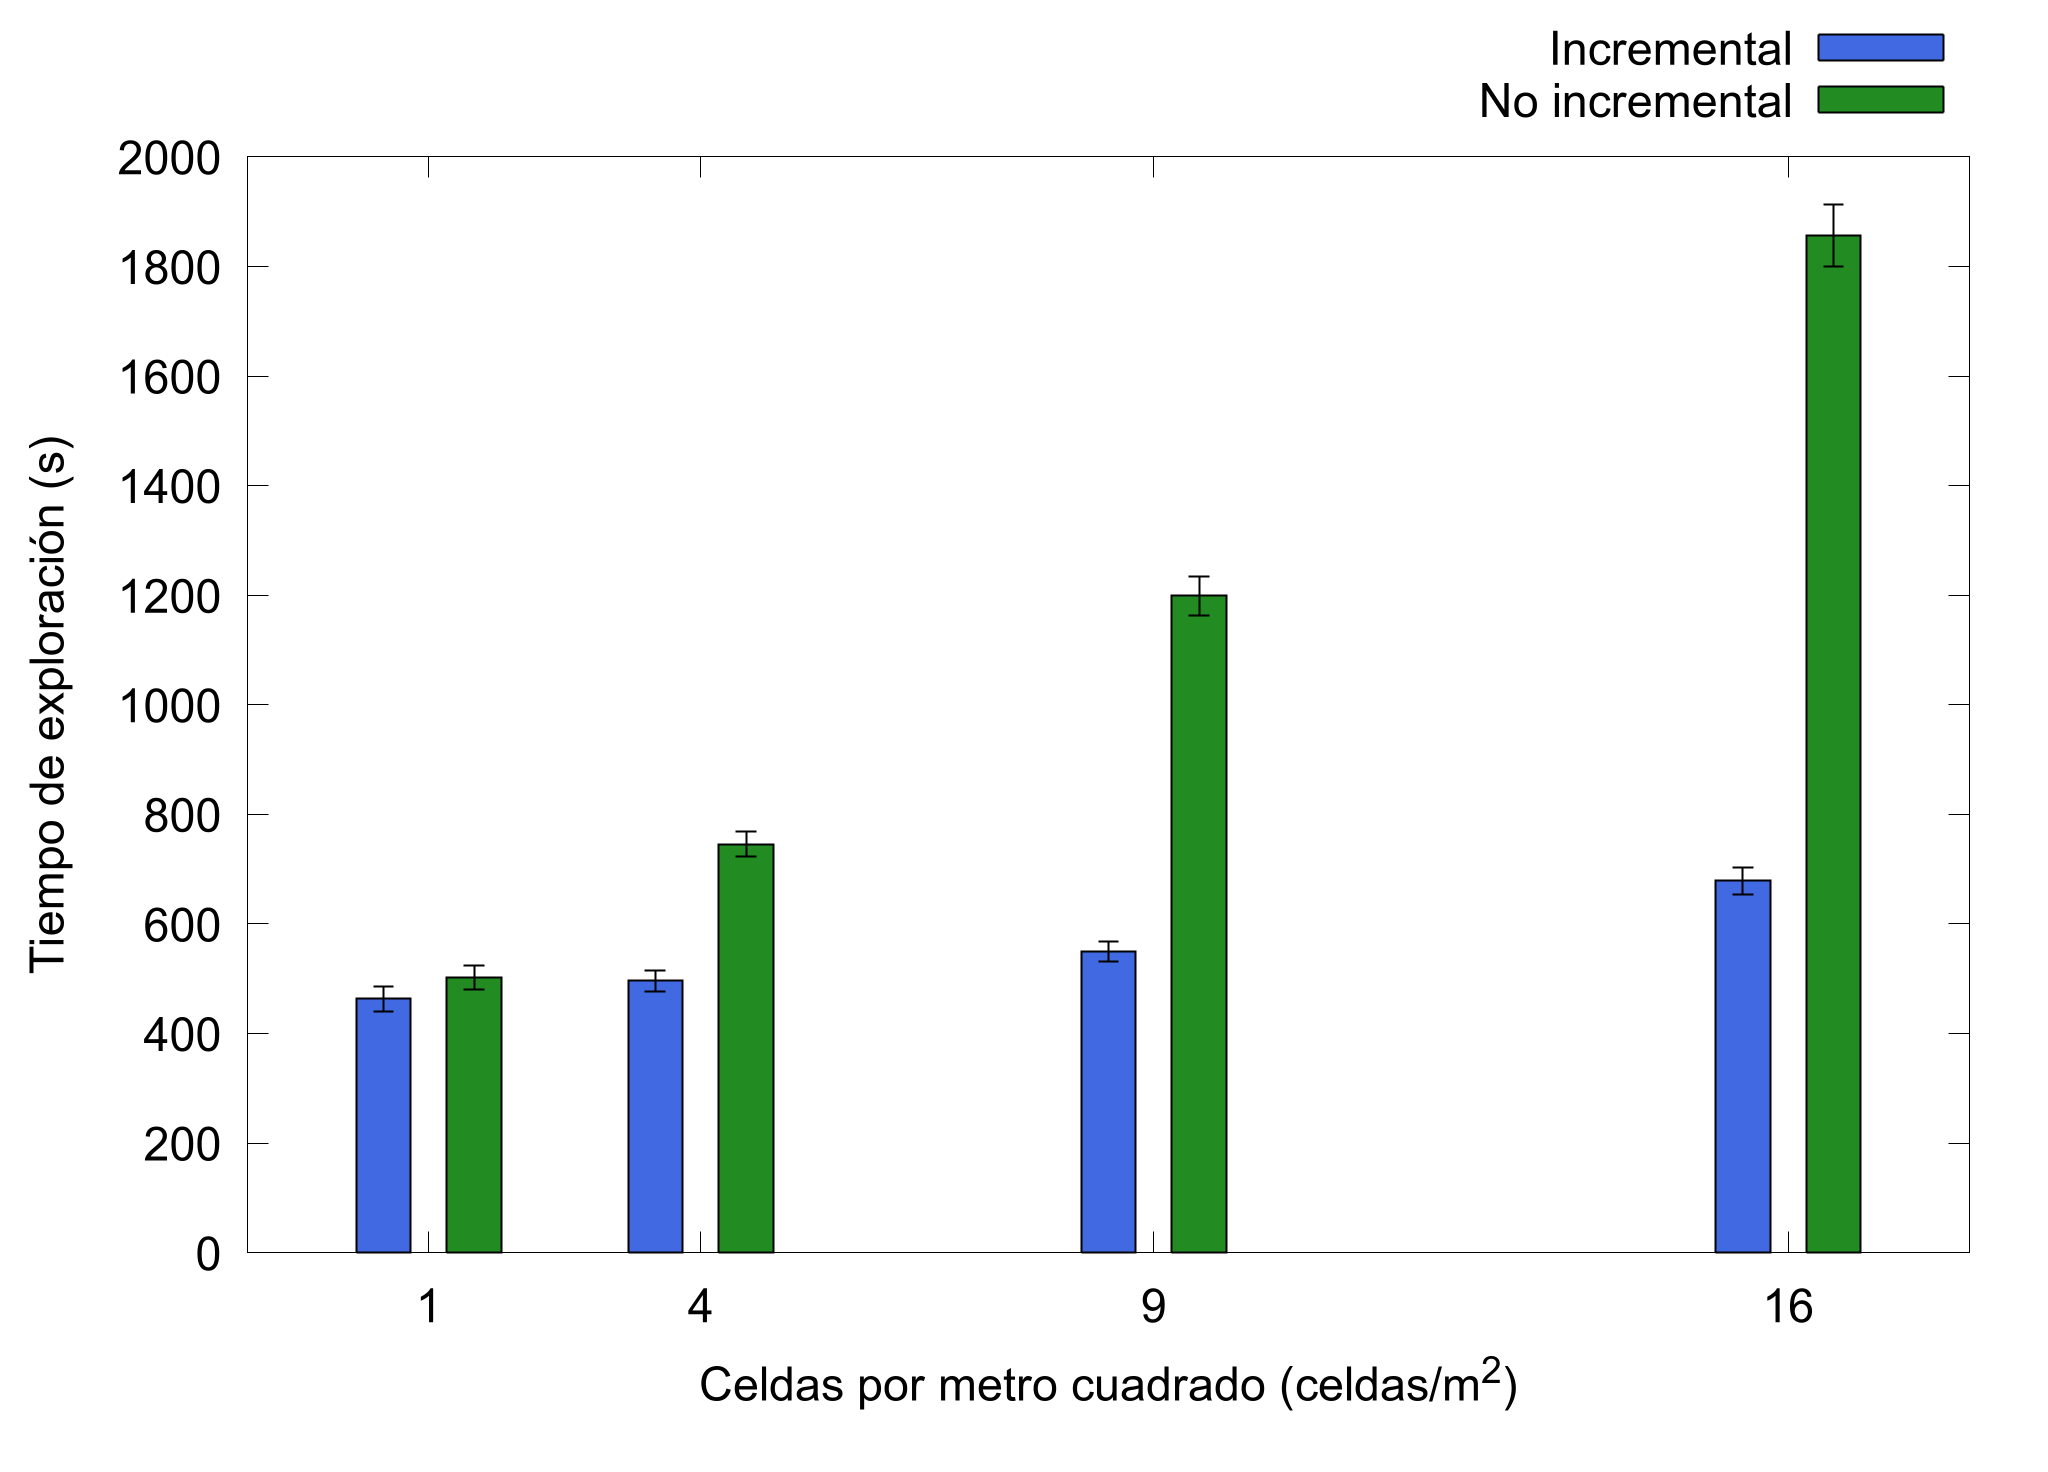
\includegraphics[clip=true, width=\graphlen]{imagenes/graficas_chicas/graficas_histo_num/incrementalidad/exploration_time.png}

  \caption{Grafica de tiempo de exploración en función de celdas por metro cuadrado.}\label{fig:gra:inc:et}

\end{figure}

\begin{figure}[H]
  \centerfloat

  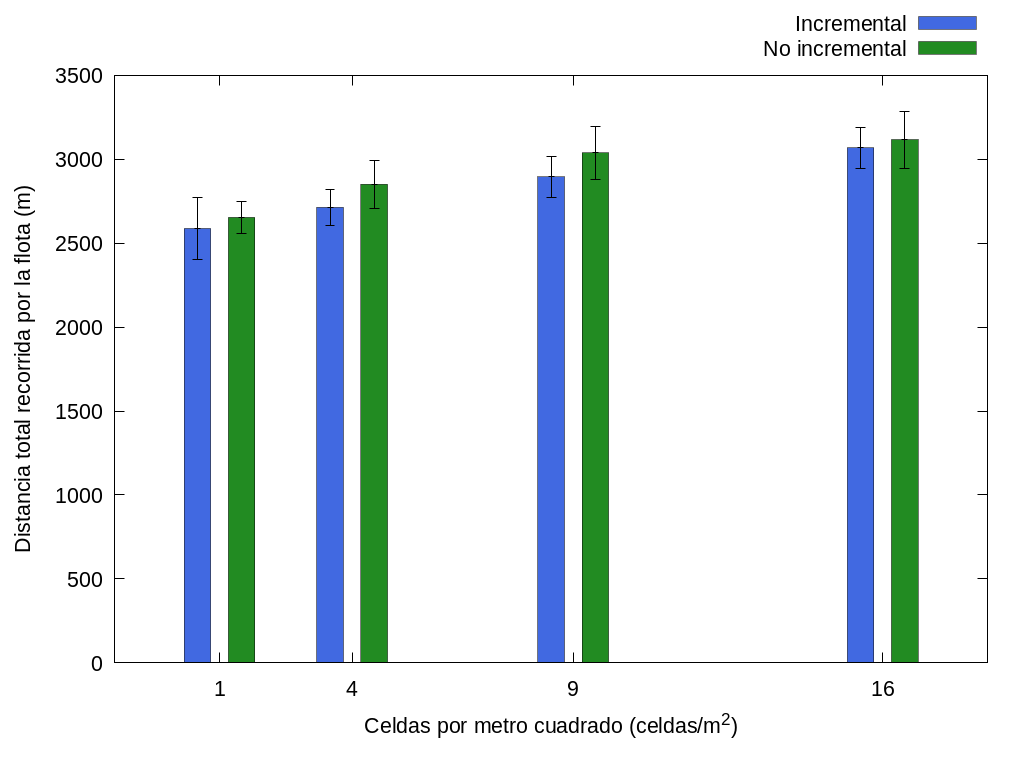
\includegraphics[clip=true, width=\graphlen]{imagenes/graficas_chicas/graficas_histo_num/incrementalidad/exploration_cost.png}

  \caption{Grafica de distancia total recorrida por la flota  en función de celdas por metro cuadrado.}\label{fig:gra:inc:ec}

\end{figure}

\begin{figure}[H]
  \centerfloat

  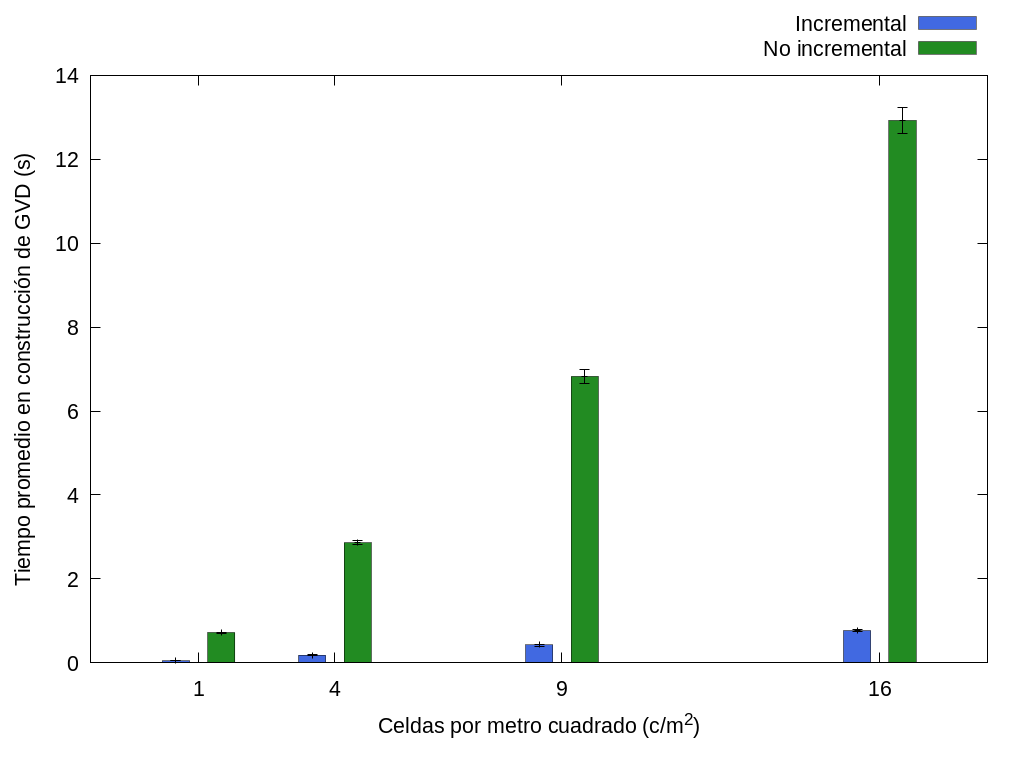
\includegraphics[clip=true, width=\graphlen]{imagenes/graficas_chicas/graficas_histo_num/incrementalidad/gvd_construction_time_mean.png}

  \caption{Grafica de la sumatoria del tiempo en construcción de GVD en función de celdas por metro cuadrado.}\label{fig:gra:inc:gvdt}

\end{figure}


\subsection{Identificación de objetivos}\label{sec:exp:idobj}
\begin{table}[H]
%24/12/2021 03:06:43
\hbadness = 10000
\tolerance=9999
\emergencystretch=10pt
\hyphenpenalty=10000
\exhyphenpenalty=100
\begin{center}

% \begin{adjustbox}{minipage=0.75\paperwidth, center}
\begin{adjustbox}{width=1\textwidth}
\small

\begin{tabularx}{\textwidth}{|X|C{0.80cm}|X|X|}

\hline
Identificación de objetivos & $\frac{celdas}{m^2}$ & Tiempo de exploración $(s)$ & Distancia total recorrida por la flota $(m)$ \\ \hline\hline
\multirow{4}{\linewidth}{\centering Simplificación de fronteras basada en cubrimiento}
& 1 & 480.8±34.7 & 2587.0±186.4\\ \cline{2-4}
& 4 & 498.0±25.3 & 2713.1±107.5\\ \cline{2-4}
& 9 & 553.4±24.9 & 2894.7±124.5\\ \cline{2-4}
& 16 & 689.7±29.0 & 3067.9±121.9\\ \hline\hline
\multirow{4}{\linewidth}{\centering Simplificación de fronteras basada en K-Means}
& 1 & 491.0±25.7 & 2628.0±98.6\\ \cline{2-4}
& 4 & 494.3±28.2 & 2684.8±106.7\\ \cline{2-4}
& 9 & 532.6±21.1 & 2813.0±96.4\\ \cline{2-4}
& 16 & 652.0±32.7 & 2962.4±136.6\\ \hline\hline
\multirow{4}{\linewidth}{\centering Fronteras sin simplificar}
& 1 & 487.9±24.3 & 2750.7±142.3\\ \cline{2-4}
& 4 & 532.8±24.7 & 3028.3±136.1\\ \cline{2-4}
& 9 & 643.3±22.8 & 3216.9±121.3\\ \cline{2-4}
& 16 & 925.8±104.7 & 3352.5±208.7\\ \hline
\end{tabularx}
\end{adjustbox}

\caption{Resultados de tiempo y costo de exploración obtenidos en las pruebas realizadas con los distintos métodos de identificación de objetivos.}
\label{tab:ident_obj1}
\end{center}

\end{table}



\begin{figure}[H]
  \centerfloat

  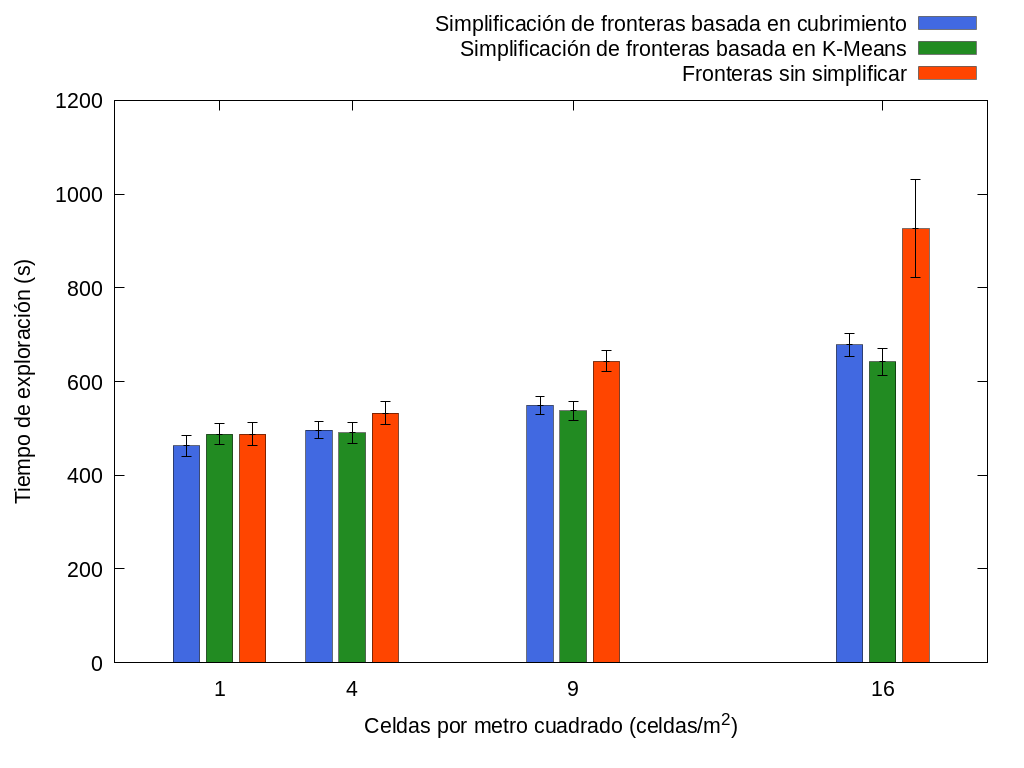
\includegraphics[clip=true, width=\graphlen]{imagenes/graficas_chicas/graficas_histo_num/ident_obj/exploration_time.png}

  \caption{Grafica de tiempo de exploración en función de celdas por metro cuadrado.}\label{fig:gra:idobj:et}

\end{figure}

\begin{figure}[H]
  \centerfloat

  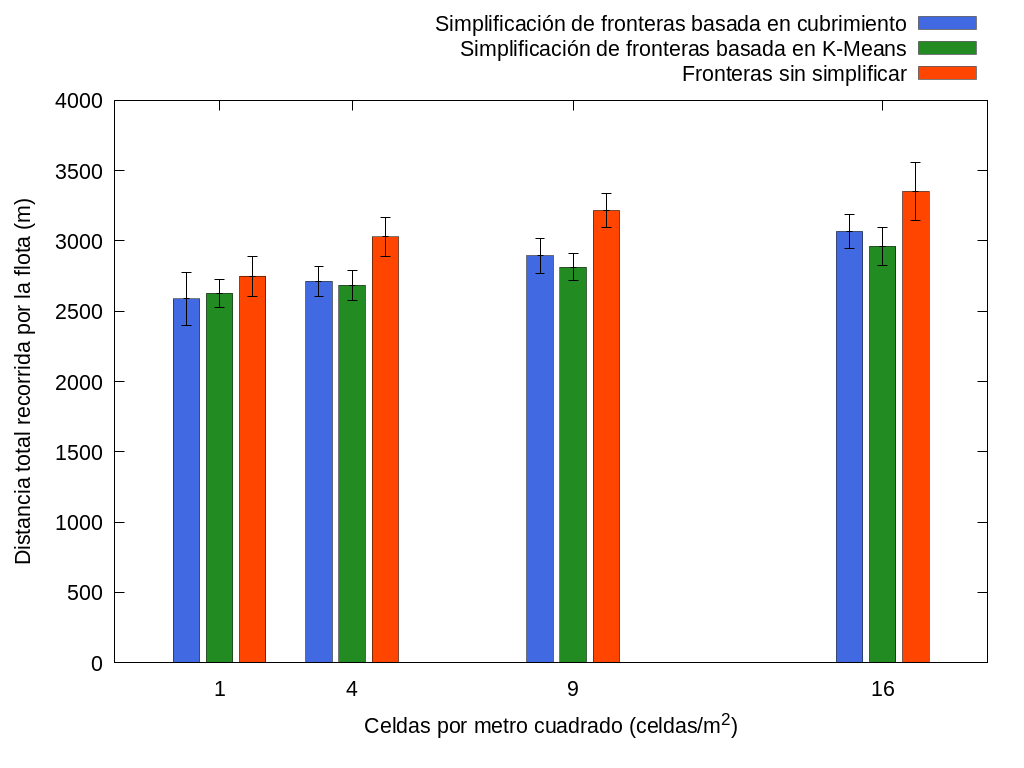
\includegraphics[clip=true, width=\graphlen]{imagenes/graficas_chicas/graficas_histo_num/ident_obj/exploration_cost.png}

  \caption{Grafica de distancia total recorrida por la flota en función de celdas por metro cuadrado.}\label{fig:gra:idobj:ec}

\end{figure}

\begin{figure}[H]
  \centerfloat

  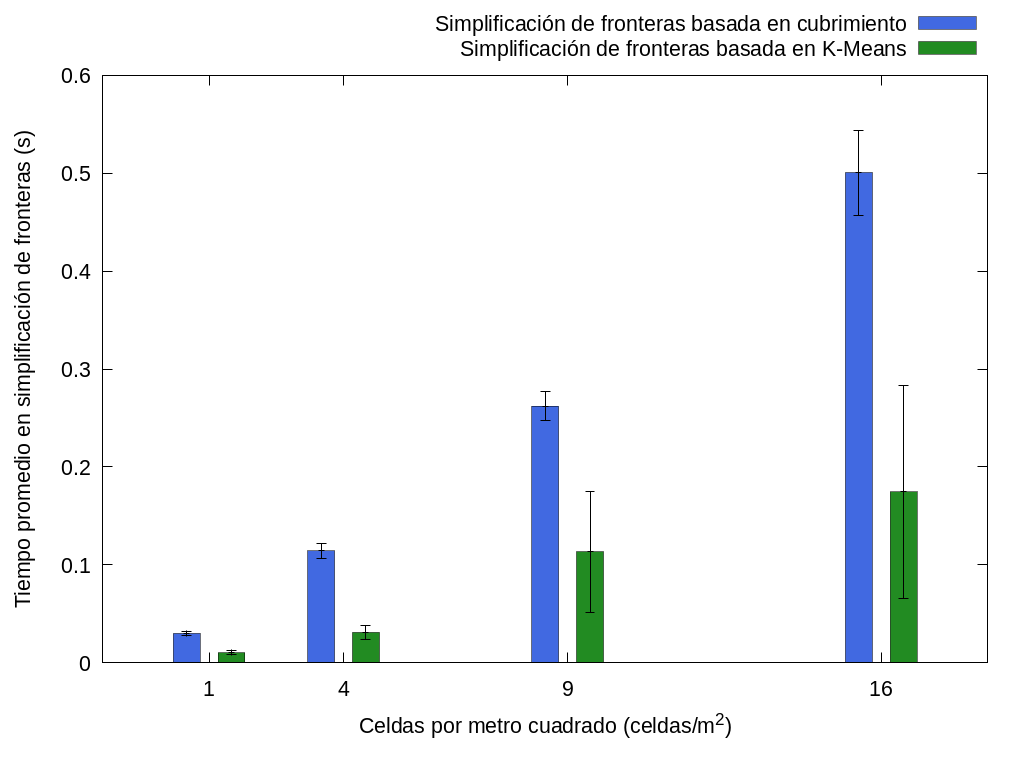
\includegraphics[clip=true, width=\graphlen]{imagenes/graficas_chicas/graficas_histo_num/ident_obj/obj_id_time_mean.png}

  \caption{Grafica de la sumatoria del tiempo en obtencion de información función de celdas por metro cuadrado.}\label{fig:gra:idobj:iobt}

\end{figure}

\subsection{Consideracion del espacio desconocido}\label{sec:exp:desco}

\begin{table}[H]
%24/12/2021 03:06:43
\hbadness = 10000
\tolerance=9999
\emergencystretch=10pt
\hyphenpenalty=10000
\exhyphenpenalty=100
\begin{center}

% \begin{adjustbox}{minipage=0.75\paperwidth, center}
\begin{adjustbox}{width=1\textwidth}
\small

\begin{tabularx}{\textwidth}{|X|C{0.80cm}|X|X|}

\hline
Consideración del espacio desconocido & $\frac{celdas}{m^2}$ & Tiempo de exploración $(s)$ & Distancia total recorrida por la flota $(m)$ \\ \hline\hline
\multirow{4}{\linewidth}{\centering Desconocidas no propagan olas y $UF \subseteq CGen$}
& 1 & 480.8±34.7 & 2587.0±186.4\\ \cline{2-4}
& 4 & 498.0±25.3 & 2713.1±107.5\\ \cline{2-4}
& 9 & 553.4±24.9 & 2894.7±124.5\\ \cline{2-4}
& 16 & 689.7±29.0 & 3067.9±121.9\\ \hline\hline
\multirow{4}{\linewidth}{\centering Desconocidas se consideran libres}
& 1 & 479.1±34.4 & 2522.2±149.5\\ \cline{2-4}
& 4 & 510.5±27.1 & 2728.9±135.2\\ \cline{2-4}
& 9 & 677.8±26.4 & 3134.2±148.8\\ \cline{2-4}
& 16 & 955.4±42.1 & 3303.6±240.5\\ \hline
\end{tabularx}
\end{adjustbox}

\caption{Resultados de tiempo y costo de exploración obtenidos en las pruebas realizadas con las distintas consideraciones del espacio desconocido al construir el GVD.}
\label{tab:desconocido1}
\end{center}

\end{table}


\begin{figure}[H]
  \centerfloat

  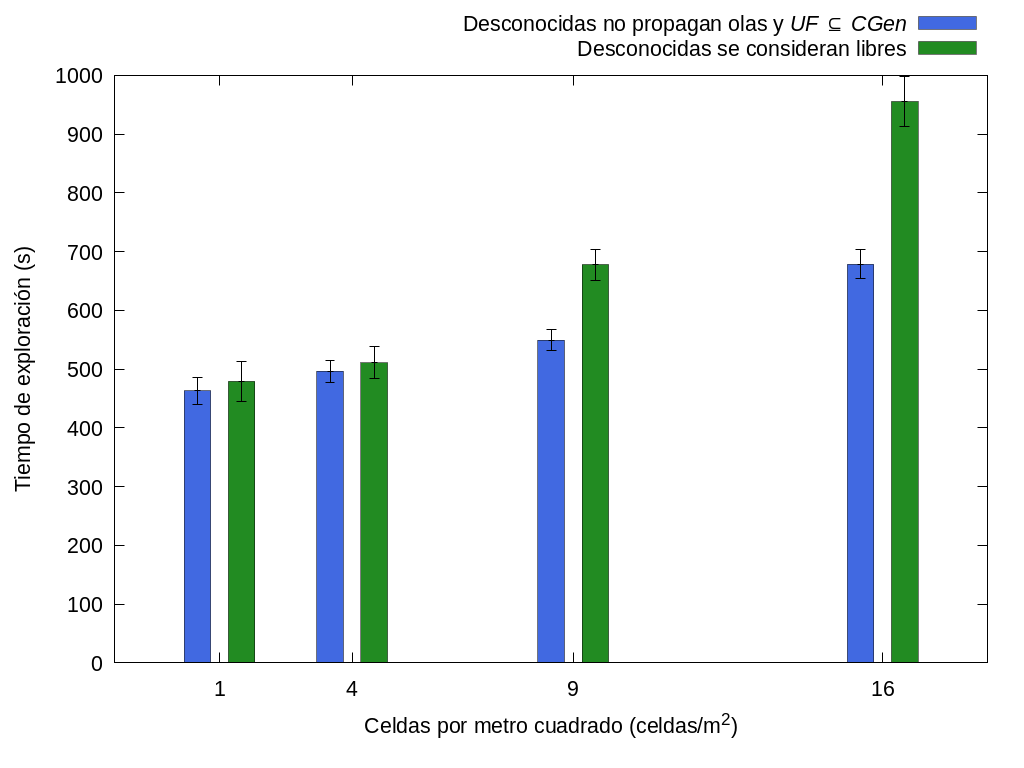
\includegraphics[clip=true, width=\graphlen]{imagenes/graficas_chicas/graficas_histo_num/desconocido/exploration_time.png}

  \caption{Grafica de tiempo de exploración en función de celdas por metro cuadrado.}\label{fig:gra:des:et}

\end{figure}

\begin{figure}[H]
  \centerfloat

  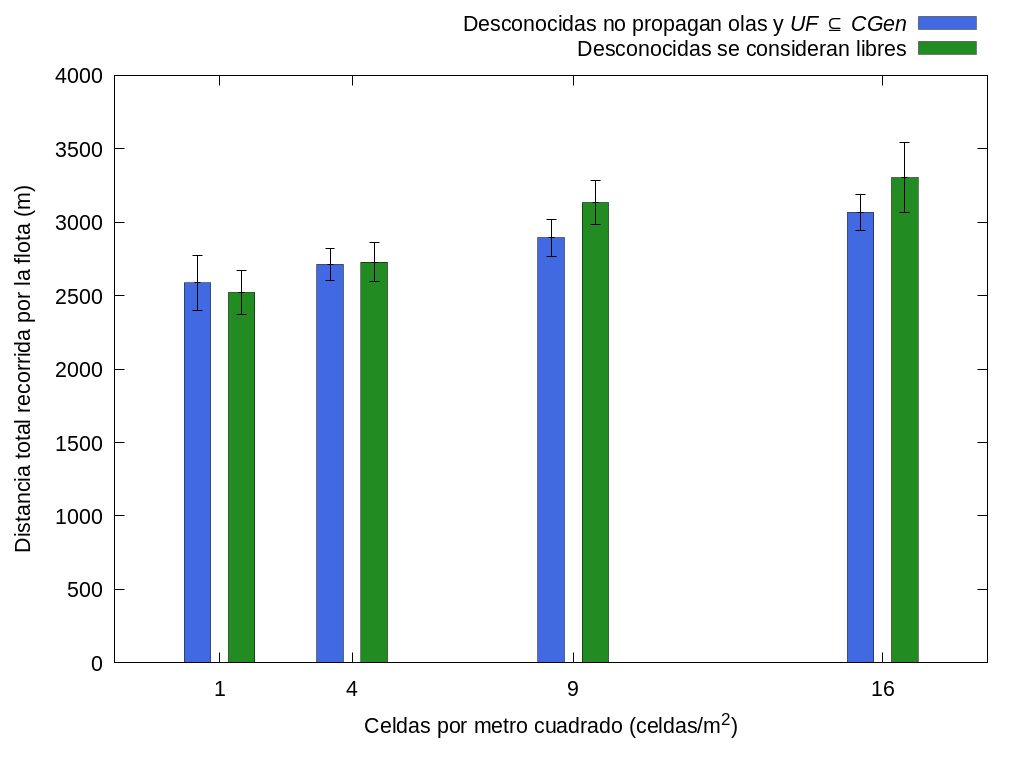
\includegraphics[clip=true, width=\graphlen]{imagenes/graficas_chicas/graficas_histo_num/desconocido/exploration_cost.png}

  \caption{Grafica de distancia total recorrida por la flota en función de celdas por metro cuadrado.}\label{fig:gra:des:ec}

\end{figure}

\begin{figure}[H]
  \centerfloat

  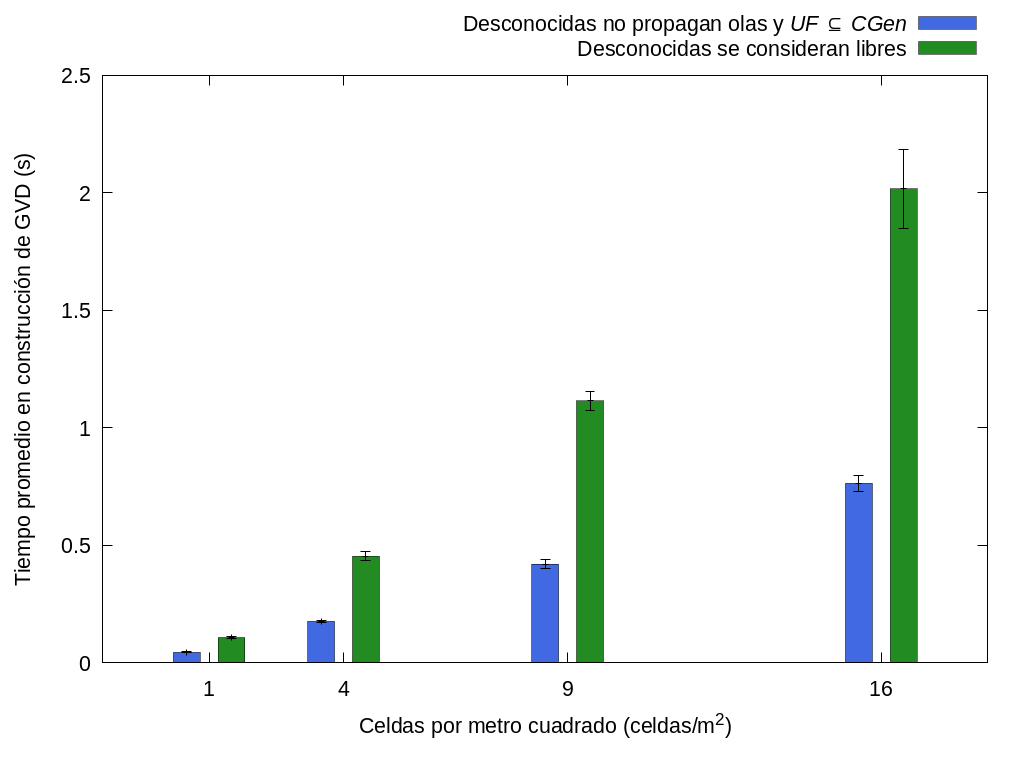
\includegraphics[clip=true, width=\graphlen]{imagenes/graficas_chicas/graficas_histo_num/desconocido/gvd_construction_time_mean.png}

  \caption{Grafica de la sumatoria del tiempo en construcción de GVD en función de celdas por metro cuadrado.}\label{fig:gra:des:gvdt}

\end{figure}

